\section{Control-Plane Scalability Bugs}

Distributed systems are full of ``control paths'' such as bootstrapping,
rebalancing, and adding/de\-com\-mission\-ing nodes (scaling out/down). These
management protocols must modify cluster-wide metadata that lives in each node
in the system (\eg, ring partition table) to decide how data flows in the
cluster. 

Our work emphasizes that scalability bugs also linger in control paths (\ie,
{\em control-plane scalability bugs}). These bugs are unfortunately often
overlooked, but yet control path correctness is crucial in today's era of
elastic cloud where cluster size is not constant all the time; rebooting,
scaling out/down, and rebalancing are common operations. We show an example of
control-plane in \sec\ref{sec-scbug}, and our observations in
\sec\ref{sec-scobs}.

\subsection{A Sample Bug}
\label{sec-scbug}

We now describe in detail a control-plane scalability bug in Cassandra,
\csb{6127} \cite{CA-One}.
%
The bug surfaced on a cluster with hundreds of nodes and led to
``\textit{\textbf{flapping}}'' nodes, a condition where node up/down status
continuously changes;  tens of thousands of flaps\footnote{A ``\textbf{flap}''
is when a node X marks a peer node Y as down.}  were observed.

\begin{figure}

\centerline{
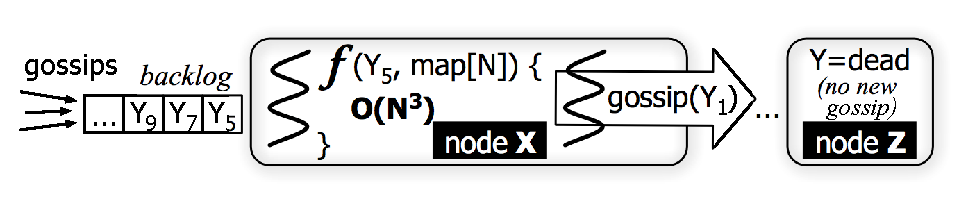
\includegraphics[height=0.8in]{F/cass1.eps}
%\includegraphics[height=0.6in]{F/empty.eps}
}
\vminfive
\mycaption[The problem of gossip-based failure detection in
Cassandra]{fig-cass1}{The problem of gossip-based failure detection in
Cassandra}{}
\vminfive
\end{figure}



To understand this bug, we need to understand the following protocols.
\begin{itemize}
\item {\bf Bootstrap:} Each node first creates partition keys (\eg, 32
random numbers) and gossips this information to peer nodes.
\item {\bf Gossip broadcast:} {\em Every second}, each node gossips to one 
random node about a list of nodes and partitions it knows (including
itself) and their {\em version} numbers.  Each node also increments its 
version number (``I'm still alive'') before gossiping.
\item {\bf Gossip processing:} The receiving node then finds any state
(metadata) differences between the two nodes to synchronize their views of
the ring.  Eventually, all nodes know about each other.
\item {\bf Failure detection:} {\em Every second}, a failure detection
daemon runs \cite{Lakshman+09-Cassandra}.  Put simply, if a node X has not 
received a new gossip about Y {\em from anyone} (Y's version has not 
changed after some period of time), X will declare Y dead (a flap).  When
X receives a new gossip about Y, it marks Y alive.
\end{itemize}

% about the bug
There are two factors that induce the bug.  The first is the {\em long latency
of scale-dependent state-update gossip processing during bootstrapping} (``f''
in Figure \ref{fig-cass1}).  While gossip processing is usually fast in a stable
cluster, it is expensive during bootstrapping as the gossips carry many new
state changes about the ring; the state-update processing time is
scale-dependent ($O(N^3)$); the larger the cluster ($N$), the larger the ring
map, the longer the processing time is.
%
This long latency is caused by {\bf (1)} state-update checkpoint to on-disk
database and {\bf (2)} multi-map cloning and updates.
%
The first one is needed for fast fault tolerance; after a node crashes, it can
reboot fast as it knows the latest view of the ring.
%
The second one is preferred for simplicity; Cassandra clones its \ts{MultiMap}
ring table and applies changes one by one to alleviate long write locks.
%
% in order to prevent a long write lock on the ring table which can block other
% user-facing protocols.

% long
The second factor is the {\em single threaded} implementation of gossip
processing.  As shown in Figure \ref{fig-cass1},  this inability to process
multiple gossips/state updates concurrently (for the sake of preventing
concurrency bugs) creates a {\em backlog} of new gossips.  For example, in {\em
every second}, Y tells someone it's alive with increasing version number (\eg,
Y$_7$), but the receiving nodes are still busy processing state changes and only
forward Y's old version number (\eg, Y$_1$).  As Y's new gossip is not
propagated on time,  other nodes (\eg, Z) will mark Y as dead.  This happens to
all nodes, not just Y.


\if 0
We mined bug repositories of four popular P2P key-value stores 
(Cassandra, Riak and 
Voldemort, Couchbase) and found \numStudy\footnote{The following are the 
  bugs we study (\textbf{with embedded hyperlinks}).
%
Cassandra: \caa, \cab, \cac, \cad, \cae ;
%
Couchbase: \cba, \cbb, \cbc, \cbd ;
%
Riak: \rka, \rkb ; and 
%
Voldemort: \vda.
%
This manual mining was arduous because there is no
standard jargon for ``scalability bugs'';
we might have missed other related bugs.
%
%For brevity, we only describe one bug in detail (\sec\ref{mot-bug})
%as the others have similar characteristics (\sec\ref{mot-observe}).
} control-plane scalability bugs.
%
These bugs caused significant availability problems such as long cluster
instability.
%
They also have complex characteristics (\sec\ref{mot-observe}).
\fi

\subsection{Observations}
\label{sec-scobs}

From the bug above, we make several important observations regarding
control-plane scalability bugs and distributed

\begin{itemize}
% only appear in large scale .. 
\item {\em Only appear at extreme scale:} \caone\ does not surface in 30-node
deployment. In 128-node cluster, the symptom appears mildly (tens of flaps).
From 200-500 nodes, flapping skyrockets to thousands of flaps. Testing in
small/medium scales is not sufficient.

% theory is not enough
\item {\em Scalable in design, but not in practice.}  Related to \caone, the
accrual failure detector \cite{Hayashibara+04-PhiFailureDetector} in
Cassandra is scalable in design \cite{Lakshman+09-Cassandra}.  However, the
design proof does not account gossip processing time, which can be long. To
understand the bug, the developers tried to ``do the [simple] math''
\cite{CA-One} but failed. In practice, new gossips are not propagated every
second (due to the backlog). The actual implementations overload gossips with
many other purposes (\eg, announcing boot/rebalance changes) beyond their
original design sketch.


% deep
\item {\em Implementation specific and hard to predict.}  The
backlog-induced flapping in \caone\ was caused specifically by Cassandra's
implementation choice: metadata checkpoint, multi-map cloning, and its
single-threaded implementation.  State-update processing time is hard to
predict (ranges from 0.001 to 4 seconds) as it depends on a 2-dimensional
input: the receiving node's ring table size and the number of new
state changes (\sec\ref{sec-eval}).

% not independent
\item {\em Cascading impacts of ``not-so-independent'' nodes.}  In
cluster-wide control protocols, distributed nodes are  not
necessarily independent; nodes must communicate with each other
to synchronize their views of cluster metadata.  As the cluster grows, the
cluster metadata size increases.  Thus, unpredictable processing time in
individual nodes can create cascading impacts to the whole cluster.

% 
\item {\em Long and difficult large-scale debugging:}
%
The bug report of \caone\ generated over 40 back-and-forth discussion
comments and took 2 months to fix.  It is apparent \cite{CA-One} that
there were many hurdles of deploying and debugging the buggy protocol at
real scale.  Important to note is that debugging is {\em not} a single
iteration; developers must {\em repeatedly} instrument the system (add
more logs) and re-run the system at scale to find and fix the bug, which
is not trivial.  The scalability bugs we studied took 6 to 157 days to
fix (27 on average).

\item {\em Not all developers have large test budgets:}
%
Another factor of delayed fixes is the lack of budget for large
test clusters.  Such luxury tends to be accessible to developers
in large companies, but not to
open-source developers.  When
\caone\ was submitted by a customer who had hundreds of nodes, the
Cassandra developers did not have an instant access to a test cluster of
the same scale.

% repeated 
\item {\em Quick fixes and repeated bugs:} Bugs are often fixed with quick
patches (development pressures), but the fix might not eradicate the problem
completely \cite{Yin+11-FixesBecomeBugs}.
%
The patch for \caone\ simply disables failure detection during bootstrap. But
the bug still appeared in another workload (\eg, scaling out from 128 to 256
nodes).
%
The simple fix has been removed later and the gossip protocol has been
redesigned.
%
And old fixes can become obsolete in protocol re-designs, which then can give
birth to new scalability bugs such as the fix for \csb{3831} became obsolete as
``vnodes'' was introduced, then led to a new scalability bug (\csb{3881}).

\end{itemize}

\subsection{State of the Art}

We now discuss popular approaches (simulation, extrapolation, and emulation) for
unearthing scalability bugs.
% ......
First, simulation approaches test system/application models in different scales
\cite{Calotoiu+13-ApmScaleBug, Laguna+15-DebugAtScale}. A model can look
scalable but the actual implementation can contain unforeseen bugs. Our
observations above accentuate the need for scale-checking distributed system
{\em implementations} at {\em real scale}.


% --------------- mini cluster
Second, extrapolation monitors system behaviors in ``mini clusters'' and 
extrapolates them to larger scales (\sec2.1 in \cite{Wang+14-Exalt}).
However, mini clusters tend to be order(s) of magnitude smaller than real
deployments.
% (\sec2.2 in \cite{Leesatapornwongsa+14-Drill}).  
% Not all
% developers have the luxury of mini clusters (\eg, ``mini'' can imply
% hundreds nodes in large companies).  
Most importantly, system behaviors do not always extrapolate linearly
\cite{Wang+14-Exalt}; for the bugs in our work (\sec\ref{sec-eval}), even an
extrapolation based on a 100-node cluster will not reveal the bug symptoms.

% --------------- emulation
Finally, real-scale emulation checks real implementations in an emulated
environment (\eg, DieCast and Exalt).
%
DieCast \cite{Gupta+08-DieCast}, invented for network emulation, can 
colocate many processes/VMs on a single machine as if they run 
individually without contention.  The trick is adding ``time dilation
factor'' (TDF) support \cite{Gupta+06-TimeDilation} into the VMM (\eg, Xen).
%
For example, TDF=5 implies that for every second of wall-clock time, each
emulated VM on the VMM believes that time has advanced by only 200 ms. 
%
The most significant drawback of DieCast is that high colocation factor
(\eg, TDF$=$100) is likely not desirable, for two reasons: prolonged
testing time (TDF$=$100 implies 100x longer run) and memory overcapacity.
%
Many distributed systems today are implemented in managed languages (\eg, Java,
Erlang) whose runtimes consume non-negligible memory overhead. Java and Erlang
VMs for example use around 70 and 64 MB of memory per process respectively. 
%
DieCast was only evaluated with TDF=10.

% co-location -- data compression -- exalt
Exalt \cite{Wang+14-Exalt} targets I/O-intensive scalability bugs.  With a
custom data compression, users' data is compressed to zero byte on disk (but the
size is recorded) while metadata is not compressed.  With this, Exalt can
co-locate 100 emulated HDFS datanodes on one machine.  In its evaluation, most
of the bugs reproduced are in the HDFS namenode which runs alone on one machine.
As the authors stated, their approach ``may not discover scalability problems
that arise at the nodes that are being emulated [the datanodes]'' (\sec4.1 in
\cite{Wang+14-Exalt}).  Thus, Exalt is not suitable for finding control-plane
scalability bugs in P2P distributed systems.

% P2P systems \cite{sosp01-past}.

% for control-plane
In summary, we did not find a fast single-machine approach that can scale-check
control-plane protocols in P2P systems.
%
The scalability bugs here are typically caused by the scale-dependent processing
time, not network or I/O bottlenecks.  As DieCast targets {\em network}
emulation via time dilation and Exalt targets {\em storage} space emulation via
compression, our work uniquely targets {\em processing time} emulation,
completing a missing piece.

